\chapter{Networking And Cryptography Tools} % (fold)
\label{cha:Networking and Cryptography tools}
	% We discuss the networking and cryptographic tools used in our work.
	% referred from \cite{menezes2010handbook,stinson2005cryptography}.
	% For example, we describe the Hash function, its properties and how it helps us achieve data integrity.

	The word cryptography means ``secret writing''.
	It is the art and science of concealing meaning.
	Cryptanalysis is the breaking of codes.
	The basic component of cryptography is a cryptosystem \cite{bishop2004introduction}.
	\begin{definition}
		A cryptosystem is a $5$-tuple ($ \mathcal{E,D,M,K,C}$), where $\mathcal{M}$ is the set of \textit{plaintexts}, $\mathcal{K}$ is the set of \textit{keys}, $\mathcal{C}$ is the set of \textit{ciphertexts}, $\mathcal{E}:\mathcal{M} \times \mathcal{K} \rightarrow \mathcal{C}$ is the set of \textit{enciphering functions}, and $\mathcal{D}:\mathcal{C} \times \mathcal{K} \rightarrow \mathcal{M}$ is the set of \textit{deciphering functions}.
	\end{definition}

\section{Symmetric Key Encryption}
	% Classical cryptosystem (also called symmetric cryptosystem or single-key cryptosystem) are cryptosystem that use the same key for encipherment and decipherement.
	% In these system, for all $E_{k} \in \mathcal{C}$ and $k \in \mathcal{K}$, there is a $D_{k} \in \mathcal{D}$ such that $D_{k} = E_{k}^{-1}$.
	% \begin{definition}
	Consider an encryption scheme consisting of the sets of encryption and decryption transformations $\{E_{e}: e \in \mathcal{K}\}$ and $\{D_{d}: d \in \mathcal{K}\}$, respectively, where $\mathcal{K}$ is the key space.
	The encryption scheme is said to be \textit{symmetric-key} if for each associated encryption/decryption key pair ($e,d$), it is computationally ``easy'' to determine $d$ knowing only $e$, and to determine $e$ from $d$ \cite{menezes2010handbook}.
	In most practical symmetric-key schemes $e = d$.
	% \end{definition}

	A two party communication using symmetric key encryption can be described by the block diagram of Figure \ref{fig:symmetric-key}. 
	One major issue with symmetric key system is to find an efficient method to agree upon and exchange keys securely, which is known as \textit{key-distribution problem}. 

	\begin{figure}[h!]
	 	\centering
	 	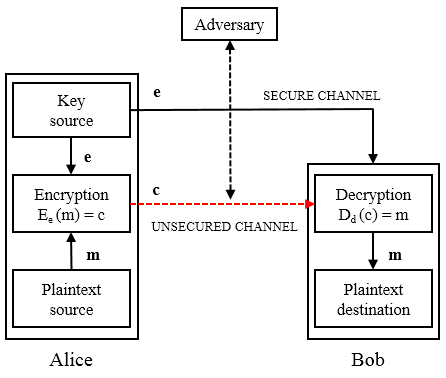
\includegraphics{images/symmetric-key.png}
	 	\caption{Two party communication using encryption, with a secure channel for key exchange. The decryption key $d$ can be efficiently computed from the encryption key $e$. }
	 	\label{fig:symmetric-key}
	 \end{figure} 

\section{Asymmetric/Public Key Encryption}
% In asymmetric or public-key cryptosystem, uses a key pair for encipherment and decipherement .
% In such systems, for all $E_{K_{1}} \in \mathcal{C}$ and $K_{1} \in \mathcal{K}$, there is a $D_{K_{2}} \in \mathcal{D}$ such that $K_{2} \in \mathcal{K}$ where $\mathcal{K} = K_{1} \times K_{2}$.
% For all $k \in \mathcal{K}$,\  there exists $(S_{k},P_{k})$ such that the following is true.
% \begin{equation}
% 	{D}(\ {E}(\ {M},\ S_{k}\ ),\ P_{k}\ ) =\ {M}
% \end{equation}
Let $\{E_{e}: e \in \mathcal{K}\}$ be a set of encryption transformations, and let $\{D_{d}: d \in \mathcal{K}\}$ be the set of corresponding decryption transformations, where $\mathcal{K}$ is the key space.
Consider any pair of associated encryption/decryption transformations $(E_{e},D_{d})$ and suppose that each pair has the property that knowing $E_{e}$ it is computationally infeasible, given a random ciphertext $c \in \mathcal{C}$, to find the message $m \in \mathcal{M}$ such that $E_{e}(m) = c$.
This property implies that given $e$ it is infeasible to determine the corresponding decryption key $d$.
This is unlike symmetric key ciphers where $e$ and $d$ are essentially the same\cite{menezes2010handbook}.

Consider the two party communication between Alice and Bob illustrated in Figure \ref{fig:public-key}. 
Bob selects the key pair $(e, d)$. 
Bob sends the encryption key $e$ (called the \textit{public key}) to Alice over any channel but keeps the decryption key $d$ (called the \textit{private key}) secure and secret.
Alice may subsequently send a message $m$ to Bob and applying the encryption transformation determined by Bob's public key to get $c = E_{e}(m)$.
Bob decrypts the ciphertext $c$ by applying the inverse transformation $D_{d}$ uniquely determined by $d$.
Here the encryption key is transmitted to Alice over an unsecured channel.
Since, the encryption key $e$ nedd not be kept secret, it may be made public.
\begin{figure}[h!]
	\centering
	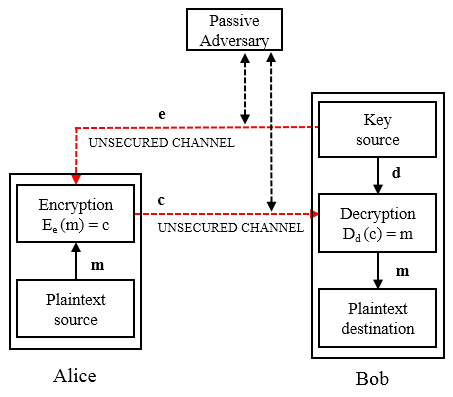
\includegraphics{images/public-key.png}
	\caption{Encryption using public key techniques}
	\label{fig:public-key}
\end{figure}

\section{Hash Function}
	A hash function takes a message as its input and outputs a fixed length message called hash code.
	The hash code represents a compact image of the message like a digital fingerprint.
	Hash functions are used to achieve data integrity.

	A hash function $h$ should have the following properties:
	\begin{itemize}
		\item Compression - $h$ maps an input $x$ of arbitrary finite bitlength, to an output $h(x)$ of fixed bitlength $n$.
		\item Ease of computation - given $h,x$ it is easy to compute $h(x)$.
		\item Preimage resistance - for all pre-specified outputs, it is computationally infeasible to find any input which hashes to that output, i.e., to find any preimage $x'$ such that $h(x') = y$ when given $y$ for which a corresponding input is not known.
		\item 2nd-preimage resistance - it is computationally infeasible to find any second input which has the same output as any specified input, i.e, given $x$, to find a 2nd-preimage $x' \neq x$ such that $h(x') = h(x)$.
		\item Collision resistance - it is computationally to find any two distinct inputs $x,x'$ which hash to the same output, i.e., such that $h(x) = h(x')$.
	\end{itemize} 

	If you want 128-bit security you should use SHA-$256$\cite{SHA256} hash algorithm as a collision resistant hash function.
	It provides 128-bit encryption which is adequate for the application.
	Birthday attacks.
	Provides sqrt security.
	% cite NIST for SHA-256

\section{Message Authentication Codes}

\section{Digital Signatures}
	\label{sec:digital-signature}
	A digital signature is a mathematical scheme for demonstrating the authenticity of a digital message. 
	A valid digital signature gives a recipient reason to believe that the message was created by a known sender, such that the sender cannot deny having sent the message (authentication and non-repudiation) and that the message was not altered in transit (integrity).
	A Digital Signature scheme consists of the following:
	\begin{enumerate}
		\item a plain text message space $\mathcal{M}$ (set of strings over alphabets)
		\item a signature space $\mathcal{S}$ (set of possible signatures)
		\item a signing key space $\mathcal{K}$ (set of possible keys for signature generation) and a verification space $\mathcal{K^{'}}$ (a set of possible verification keys)
		\item an efficient key generation algorithm \textsf{Gen} : $N \rightarrow$ $\mathcal{K} \times \mathcal{K^{'}} $ 
		\item an efficient signing algorithm \textsf{Sign} : $ \mathcal{M} \times \mathcal{K} \rightarrow \mathcal{S}$
		\item an efficient verification algorithm \textsf{Verify} : $\mathcal{S} \times \mathcal{M} \rightarrow$ \{true, false\} 
	\end{enumerate}
	For any secret key $s_{k} \in \mathcal{K}$ and any $m \in \mathcal{M}$,	the message $m$ is signed using key $s_{k}$ as follows:
		\begin{equation}
			s = \textsf{Sign}_{s_{k}}(m)
			\label{eq:signature}
		\end{equation}
	For any $s_{k}$ let $p_{k}$ denote public key and for all $m \in \mathcal{M}$ and $s \in \mathcal{S}$, $s$ as follows:
	\begin{equation}
		\textsf{Verify}_{p_{k}}(m,s) = 
		\begin{cases}
		 \textbf{true}\ \mbox{with probability of 1} & \mbox{if}\ s = \textsf{Sign}_{s_{k}}(m)\\
		 \textbf{false}\ \mbox{with overwhelming probability} & \mbox{if}\ s \neq \textsf{Sign}_{s_{k}}(m)
		\end{cases}
		\label{eq:verification}
	\end{equation}
	where the probability space is determine by the $\mathcal {M, S, K, K^{'}}$ and perhaps the signing and verification algorithms.
	The ``overwhelming probability'' for the signature scheme determines the probability that the scheme allows for a forgery.
	Note that the Digital Signature scheme satisfies the following requirements:
		\begin{itemize}
			\item Only the owner of the secret key can generate a valid signature.
			\item The digital signature is easily verified by other parties as long as they know the public key.
			\item The digital signature is not only tied to the signer but also to the message that is being signed.
			\item Digital signatures do not encrypt the message. However, if necessary, a signed message can be encrypted after it is signed.
		\end{itemize}
	In Figure \ref{fig:digita-signature}, we show the steps for signing and verifying the hashed message \cite{DigitalSignature}. 
	\begin{figure}[h!]
		\centering
		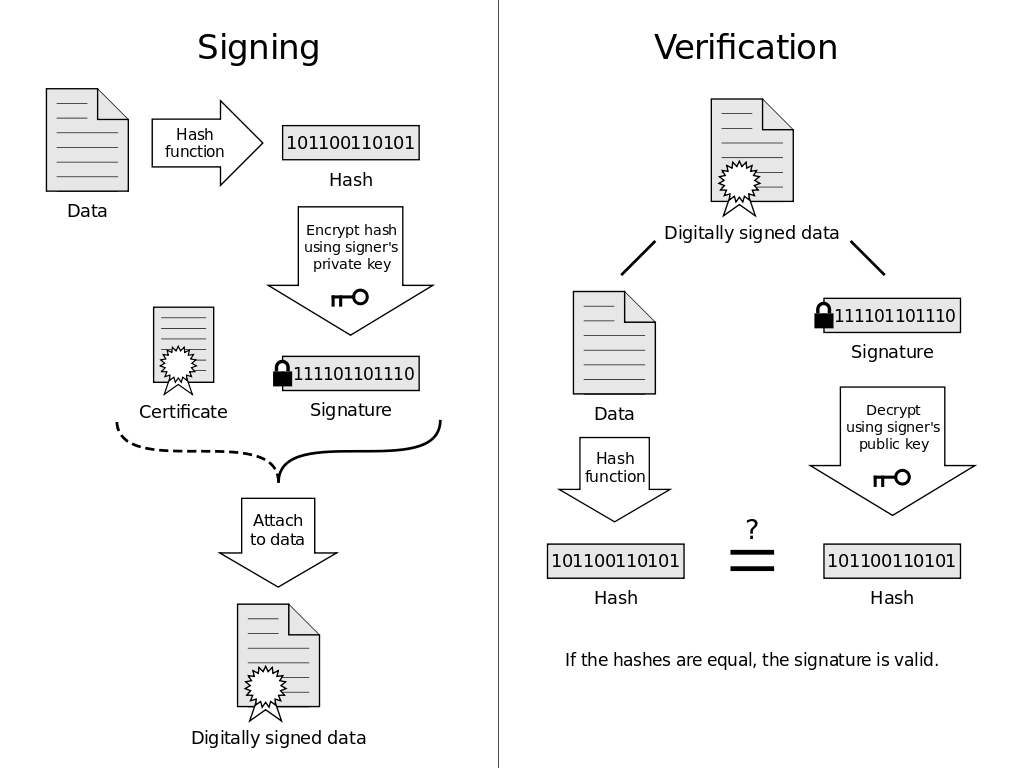
\includegraphics[scale = 0.4]{images/Digital_Signature_diagram.png}
		\caption{ Signing and verification of digital signatures}
		\label{fig:digita-signature}
	\end{figure}
	The message is hashed before its being signed to reduce the message size. 
	If the message is not hashed before signing then the signature can be longer than the message which is problematic for the longer messages.
	\textbf{Talk about non-repudiation, authenticity, integrity.}
	\textbf{Talk about similarities and differences between physical world signature non-repudiation, authenticity, integrity.}
	In physical world, your signatures are the same for all the messages. 
	But this can not be possibly true for digital signatures as the attacker can obtain one signature and then use the same signature to pretend some one else.


	Three different integrity-protection mechanisms HASH, MAC, Signature can be summarized in a matrix like Table \ref{table:summary} \cite{2002-Stajano-ubiquitous}.
	The main difference between the various primitives stems from identifying who can generate the code and who can verify it.
	This determines the suitability of the construction for a given purpose.
	\begin{table}[!htb]	
		\begin{center}
			\begin{tabular}{ |l| l| l| }
		    \hline
		     & Who can generate it & Who can verify it \\
		    \hline
		    Hash & Everyone & Everyone \\	
		    \hline
		    MAC & Holders of secret & Holders of secret \\
		    \hline
		    Signature & Holder of secret & Everyone \\
		    \hline
			\end{tabular}
		\end{center}
		\caption{A comparison of integrity-protecting primitives}
	  \label{table:summary}
	\end{table}

\section {Tree generation algorithms}

\section{XOR function}

\section{Elliptic curve}